\section{Performance- und Konformitätsanalyse}
\label{sec:performance}

Aufbauend auf dem in \autoref{sec:prozessfluss} rekonstruierten Prozessfluss untersucht dieses Kapitel die Prozessleistung und -konformität:
Wie lange dauern die Prozessinstanzen, wo entstehen operative Engpässe, wie häufig und warum werden Anträge abgelehnt und an welchen Stellen
weicht das beobachtete Verhalten vom erwarteten Ablauf ab. Die Untersuchung stützt sich auf die Standard-Analysen
der Celonis-Process-Analytics-Umgebung (\textit{Process Overview}, \textit{Throughput Times}, \textit{Conformance} und \textit{Process AI})
sowie auf eigens erstellte interaktive Analyse-Views (\textit{Case Explorer}, \textit{Variant Explorer} und \textit{Rejections Dashboard}),
deren Kennzahlen über die Process Query Language (PQL) aggregiert werden \parencite{vogelgesang_celonis_2022}. Zur methodischen Validierung
werden die Ergebnisse an zentralen Stellen den Python-Auswertungen mit PM4Py gegenübergestellt \parencite{berti_process_2019}. \autoref{tab:kpi_comparison}
fasst die wichtigsten Performance- und Konformitätskennzahlen beider Event-Logs zusammen.

\begin{table}[htbp]
\centering
\caption{Zentrale Performance- und Konformitätskennzahlen (Celonis)}
\label{tab:kpi_comparison}
\small
\begin{tabular*}{\textwidth}{@{\extracolsep{\fill}} l c c @{}}
\toprule
\textbf{Kennzahl} & \textbf{Domestic} & \textbf{International} \\ \midrule
Cases gesamt & 10.500 & 6.449 \\
Ø Durchlaufzeit Happy Path (Median) & 9\,d (7\,d) & 66\,d (55\,d) \\
Ø Durchlaufzeit alle Cases ohne Extreme (Median) & 9\,d (7\,d) & 75\,d (66\,d) \\
Ø Durchlaufzeit alle Cases inkl.\ Extreme & 11,5\,d (bis 469\,d) & 86\,d (bis 743\,d) \\
Ø Dauer Deklarationsteil (\texttt{SUBMITTED} $\rightarrow$ \texttt{Payment}) & 11,6\,d (Median: 7,4\,d) & 14,6\,d (Median: 10,2\,d) \\
Konforme Cases: Striktes Modell (nur Variante 1) & 43,98\,\% (4.618) & 21,23\,\% (1.369) \\
Konforme Cases: Erweitertes Modell (Top-3-Varianten) & 81,00\,\% (8.470) & 38,30\,\% (2.470) \\
Verletzungstypen (im erweiterten Modell) & 19 & 56 \\
Ø Durchlaufzeit konform vs.\ verletzend (erw.\ Modell) & 10,4 vs.\ 16,3\,d (+5,9\,d) & 69,3 vs.\ 97,1\,d (+27,8\,d) \\
Schritte pro Case konform vs.\ verletzend (erw.\ Modell) & 5,1 vs.\ 6,4 & 10,2 vs.\ 11,8 \\
Cases mit mindestens einer Ablehnung (Gesamtquote) & 1.301 (12\,\%) & 1.755 (27\,\%) \\
\quad davon \texttt{Declaration REJECTED by EMPLOYEE} & 1.212 (12\,\%), +9\,d & 1.483 (23\,\%), +18\,d \\
\quad davon \texttt{Declaration REJECTED by ADMINISTRATION} & 846 (8\,\%), +11\,d & 1.287 (20\,\%), +15\,d \\
\quad davon \texttt{Declaration REJECTED by SUPERVISOR} & 281 (3\,\%), +9\,d & 211 (3\,\%), +12\,d \\
Wiederholte Einreichung (\texttt{SUBMITTED} $\rightarrow$ \texttt{SUBMITTED}) & 776 (7\,\%), +12\,d & 1.225 (19\,\%), +20\,d \\ \bottomrule
\end{tabular*}
\end{table}

% ==================================================================
\subsection{Durchlaufzeiten und Extremwertanalyse}
\label{sec:durchlaufzeiten}

\paragraph{International.} Die arithmetische Gesamtdurchlaufzeit vom ersten bis zum letzten Event eines internationalen Abrechnungsfalls beträgt 86 Kalendertage.
Wie das Histogramm in \autoref{fig:tpt_verteilung} zeigt, ist die Verteilung stark rechtsschief: Während sich die Mehrheit der Fälle (rund 4.200 Cases) in den
ersten drei Intervallen zwischen 7 und 86 Tagen konzentriert, fällt die Häufigkeit danach kontinuierlich ab, mündet jedoch am rechten Rand in einer Sammelklasse
extremer Ausreißer von 224 bis zu 743 Tagen (rund 360 Cases). Dieser ausgeprägte \textit{Long Tail} zieht das arithmetische Mittel signifikant nach oben.
In den Standard-Dashboards von Celonis werden daher drei unterschiedlich aggregierte Durchschnittswerte ausgewiesen, die analytisch strikt zu trennen sind:

\begin{itemize}[noitemsep]
	\item \textbf{86 Tage:} ungefiltertes arithmetisches Mittel \emph{aller} 6.449 Cases inklusive sämtlicher Ausreißer (Tab \textit{Throughput Times} in Process Overview),
	\item \textbf{75 Tage:} getrimmtes Mittel aller Cases \emph{ohne Extremwerte} (View \textit{Process Overview}),
	\item \textbf{66 Tage:} arithmetisches Mittel ausschließlich der 1.369 Happy-Path-Cases (Variante 1).
\end{itemize}

Für eine gegenüber Ausreißern robuste Bewertung ist der Median heranzuziehen:
Dieser liegt über alle internationalen Fälle hinweg bei 66 Tagen und reduziert sich für die Fälle auf dem Happy Path auf 55 Tage.

\paragraph{Domestic und 0-ms-Anomalie.} Inländische Deklarationen werden um ein Vielfaches schneller abgewickelt. Sowohl auf dem Happy Path als
auch im getrimmten Gesamtdurchschnitt beträgt die mittlere Durchlaufzeit 9 Kalendertage, sodass der Großteil der Erstattungen innerhalb von knapp
zwei Wochen abgeschlossen ist.

Eine gezielte Untersuchung der Varianten-Tabelle im selbsterstellten Celonis-View (\autoref{fig:view_variants} im Anhang) deckt jedoch zwei extreme
Auffälligkeiten an den Rändern der Verteilung auf:
\begin{enumerate}[noitemsep]
	\item \textbf{Fälle mit 0\,ms Durchlaufzeit (Variante 8):} Exakt 134 Domestic-Cases (1\,\%) weisen eine gemessene Durchlaufzeit von 0 Millisekunden auf. Eine Einzelfallprüfung im \textit{Case Explorer} zeigt, dass diese Traces aus lediglich einem einzigen Event (\texttt{Declaration SAVED by EMPLOYEE}) bestehen. Fachlich handelt es sich um Entwürfe, die von Mitarbeitenden im System zwischengespeichert, aber nie formal eingereicht wurden. Verbleiben diese unvollständigen Instanzen ungefiltert im Log, verzerren sie sowohl die durchschnittliche Durchlaufzeit als auch die Schrittanzahl künstlich nach unten.
	\item \textbf{Extreme Langläufer durch Liegezeiten (bis 283 Tage):} Am oberen Ende finden sich auch im Domestic-Log gravierende Ausreißer. Eine im \textit{Case Explorer} durchgeführte Einzelfallanalyse des Extremfalls \texttt{f954cbea-975d-4cf4-a1f6-a400d81f0d9f} (Durchlaufzeit: 283 Tage, 9 Aktivitäten; siehe \autoref{fig:case_f954} im Anhang) verdeutlicht die Ursache: Nachdem die Erklärung am 04.12.2017 eingereicht wurde, verblieb sie fast neun Monate ohne jegliche Systemaktivität, ehe sie am 27.08.2018 von der Administration abgelehnt wurde. Nach der erneuten Einreichung am 10.09.2018 wurde der gesamte restliche Freigabe- und Auszahlungsprozess (inklusive Budget Owner und Supervisor) innerhalb von nur drei Tagen bis zum 13.09.2018 abgeschlossen. Die extremen Durchlaufzeiten resultieren folglich nicht aus komplexen Bearbeitungen, sondern aus monatelang verwaisten Anträgen, die zudem jahresübergreifende Events erzeugen.
\end{enumerate}

\paragraph{Vergleichbarkeit der beiden Logs.}
Die Gesamtdurchlaufzeiten von rund 9 Tagen (Domestic) und 66 bzw.\ 86 Tagen (International) lassen sich nicht direkt miteinander vergleichen, da beide Logs unterschiedliche Prozessgrenzen abbilden: Während ein Domestic-Case erst mit \texttt{Declaration SUBMITTED by EMPLOYEE} startet, umfasst ein International-Case zusätzlich die gesamte Permit- und Reisephase. Um einen methodisch fairen Vergleich herzustellen, wurde im eigens erstellten Analyse-Tab \textit{TPT Analysis} exakt derselbe Prozessabschnitt vom ersten Einreichen der Erklärung (\texttt{Declaration SUBMITTED by EMPLOYEE}, \textit{First}) bis zum Zahlungsabschluss (\texttt{Payment Handled}, \textit{Last}) für beide Logs isoliert ausgewertet (\autoref{fig:view_compare_dec}).

Das Ergebnis relativiert den scheinbar massiven Geschwindigkeitsunterschied erheblich: Im Domestic-Log benötigt dieser Abschnitt über alle ausgezahlten Fälle hinweg im ungetrimmten Mittel 11,6 Tage bei einem Median von 7,41 Tagen (Minimum: 1,06 Tage, Maximum: 368 Tage). Im International-Log liegt das arithmetische Mittel für denselben Abschnitt bei 14,6 Tagen und der Median bei 10,2 Tagen (Minimum: 1,09 Tage, Maximum: 429 Tage). Die eigentliche Prüfung, Freigabe und Auszahlung einer Auslandsabrechnung dauert im Schnitt folglich nur rund 3,0 Tage (im Median 2,8 Tage) länger als bei einer Inlandsreise – ein moderater Aufschlag, der sich durch die höhere Komplexität ausländischer Belege und die höhere Korrekturquote erklärt. Die übrigen mehr als 70 Tage Differenz in der Gesamtdurchlaufzeit entfallen vollständig auf die vorgelagerte Permit-Genehmigung, die Buchungsvorlaufzeit, die Reisedauer sowie das verzögerte Einreichen nach Rückkehr.

\begin{figure}[htbp]
	\centering
	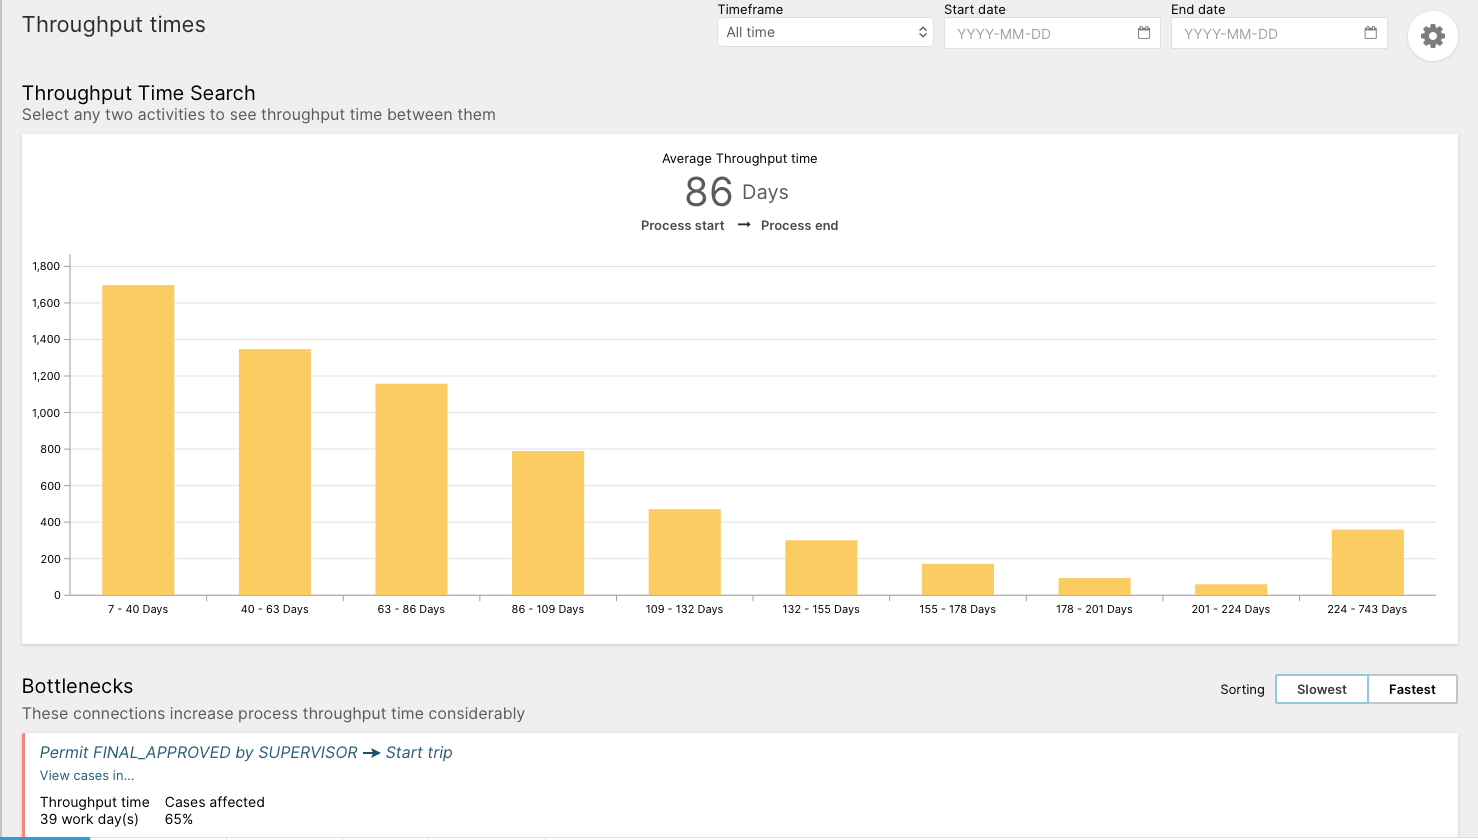
\includegraphics[width=0.85\textwidth]{figures/celonis/int_throughput.png}
	\caption{Rechtsschiefe Verteilung der Durchlaufzeiten mit Long Tail bis 743 Tage (International, Celonis \textit{Throughput Times})}
	\label{fig:tpt_verteilung}
\end{figure}

\paragraph{Zeitliche Muster.} Die Anzahl neu gestarteter Fälle pro Monat unterliegt im Beobachtungszeitraum einem markanten Strukturbruch. Im International-Log starten im Jahr 2017 durchschnittlich rund 10 Cases pro Tag; ab Januar 2018 vervielfacht sich dieser Wert sprunghaft auf bis zu 55 Starts pro Tag im April 2018. Dasselbe Muster zeigt sich im Domestic-Log mit 2.240 Case-Starts im Jahr 2017 gegenüber 8.345 im Jahr 2018 (\autoref{tab:basisstatistik}). Wie in \autoref{sec:einleitung} erläutert, ist dieser Anstieg kein Ausdruck einer veränderten Reisetätigkeit, sondern das direkte Resultat des universitätsweiten System-Rollouts Anfang 2018 \parencite{van_dongen_bpi_2020}. Ab Anfang 2019 (301 Domestic- bzw.\ 176 International-Starts) läuft die Erfassung neuer Fälle aus, während einzelne Bearbeitungs-Events bis 2020 nachlaufen. Methodisch führt dies an den Rändern des Beobachtungsfensters zu einer statistischen Verzerrung: Fälle aus 2017 hatten bis zum Datenexport über zwei Jahre Zeit, um selbst extremste Liegezeiten (wie im obigen 283-Tage-Fall) vollständig im Log abzubilden, wohingegen spät im Jahr 2018 gestartete Fälle bei einer kurzen Abwicklung bevorzugt im Log abgeschlossen sind (Rechtszensierung langer Fälle).

% ==================================================================
\subsection{Bottlenecks}
\label{sec:bottlenecks}

Die Bottleneck-Analyse in Celonis identifiziert diejenigen direkten Aktivitätsübergänge, welche die Gesamtdurchlaufzeit am stärksten verzögern (\autoref{fig:bottlenecks}).

\paragraph{Domestic.} Innerhalb des Genehmigungsworkflows sind die Liegezeiten mit ein bis zwei Arbeitstagen ausgesprochen kurz. Die beiden gravierendsten Engpässe treten erst nach Abschluss sämtlicher inhaltlicher Prüfungen in der finalen Zahlungsabwicklung auf: Der Übergang \texttt{FINAL\_APPROVED by SUPERVISOR \textrightarrow\ Request Payment} beansprucht im Mittel 3 Arbeitstage (96\,\% der Cases), gefolgt von \texttt{Request Payment \textrightarrow\ Payment Handled} mit weiteren 4 Arbeitstagen (95\,\% der Cases). Damit entfallen rund sieben Arbeitstage – und somit der überwiegende Teil der neuntägigen Happy-Path-Durchlaufzeit – auf die rein technische Auszahlungsphase. Da diese Aktivitäten vom Akteur \texttt{SYSTEM} ausgeführt werden, deutet dieses Muster stark darauf hin, dass Zahlungsanweisungen und Überweisungsläufe im Finanzsystem der Universität nicht in Echtzeit, sondern gebündelt in wöchentlichen oder halbwöchentlichen Batch-Läufen prozessiert werden. Als drittgrößter Verzögerungsfaktor erweist sich der Übergang \texttt{APPROVED by BUDGET OWNER \textrightarrow\ FINAL\_APPROVED by SUPERVISOR} (3\,AT in 26\,\% der Cases), was bestätigt, dass die zusätzliche Hierarchiestufe des Budgetverantwortlichen die Prozessdauer spürbar erhöht.

\paragraph{International.} Im Auslandsprozess weist Celonis rechnerisch den Übergang \texttt{Permit FINAL\_APPROVED by SUPERVISOR \textrightarrow\ Start trip} mit 39 Arbeitstagen (65\,\% der Cases) als langsamsten Prozessschritt aus. Fachlich stellt diese Zeitspanne jedoch keinen operativen Prozessengpass dar, sondern spiegelt die notwendige und erwünschte Vorlaufzeit zwischen der Genehmigung einer Auslandsdienstreise und dem tatsächlichen Reiseantritt wider. Analog bildet der Übergang \texttt{Start trip \textrightarrow\ End trip} (5\,AT, 90\,\%) schlicht die physische Dauer der Dienstreise ab. Dies unterstreicht, dass algorithmisch identifizierte Liegezeiten im Process Mining stets im fachlichen Domänenkontext interpretiert werden müssen.

Der tatsächliche operative Flaschenhals im International-Log liegt im Übergang \texttt{End trip \textrightarrow\ Declaration SUBMITTED by EMPLOYEE}, der bei 71\,\% der Fälle im Mittel 13 Arbeitstage (rund drei Kalenderwochen) beansprucht. Diese Verzögerung entsteht vollständig aufseiten der reisenden Mitarbeitenden, die ihre Belege nach Rückkehr erst mit erheblichem Verzug einreichen. Die nachgelagerte Zahlungsphase (\texttt{Request Payment \textrightarrow\ Payment Handled}, 3\,AT, 95\,\%) verhält sich hingegen konsistent zum Inlandsprozess. Auffällig ist zudem der zweitlangsamste Übergang \texttt{Permit FINAL\_APPROVED by SUPERVISOR \textrightarrow\ Declaration SUBMITTED by EMPLOYEE} (17\,AT, 12\,\% der Cases), bei dem die Reise-Events zwischen Permit-Freigabe und Kostenerklärung komplett fehlen; diese Konformitätsanomalie wird in \autoref{sec:unerwartet} aufgelöst.

\begin{figure}[htbp]
	\centering
	\begin{subfigure}[t]{0.49\textwidth}
		\centering
		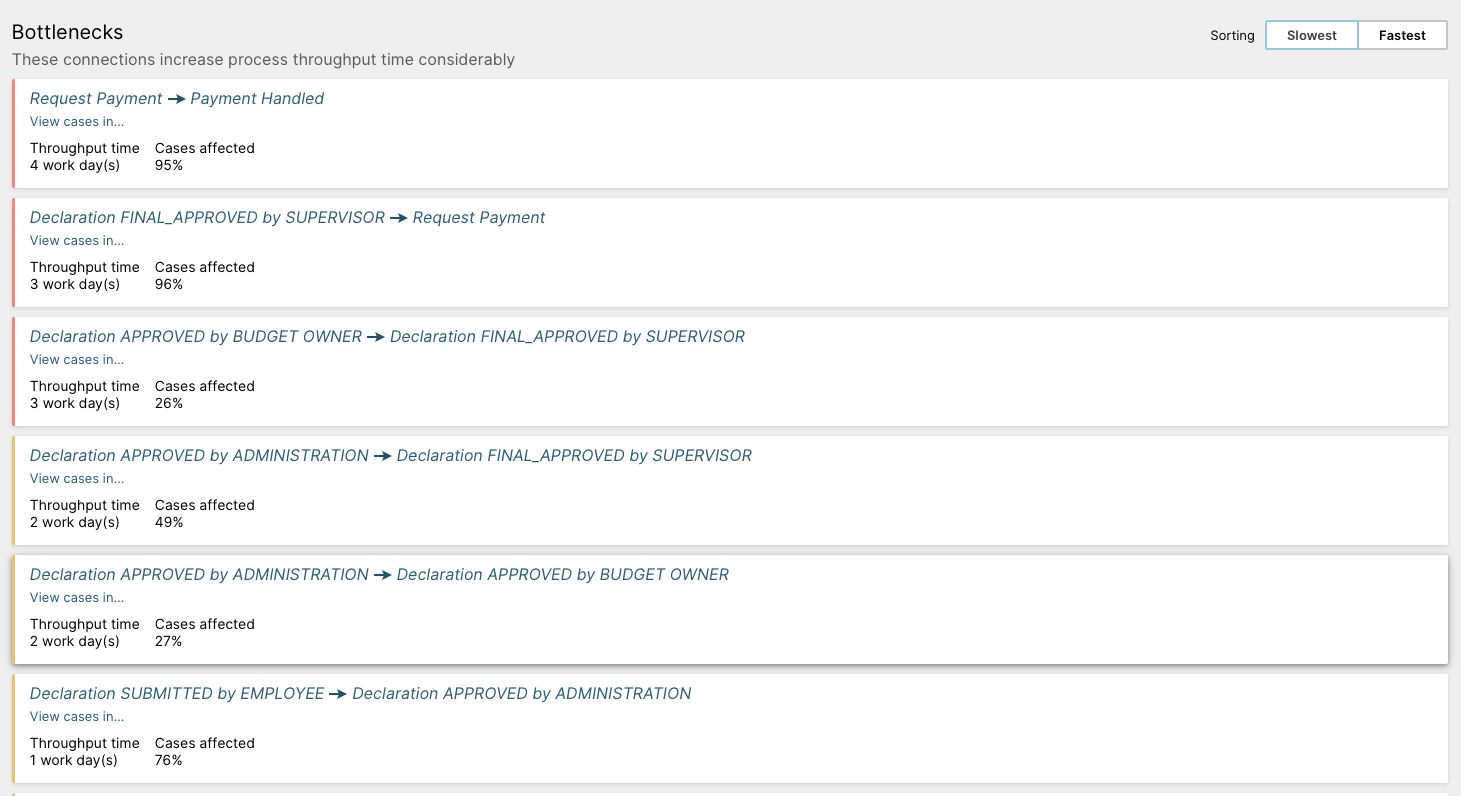
\includegraphics[width=\textwidth]{figures/celonis/dom_bottlenecks.png}
		\caption{Domestic}
	\end{subfigure}
	\hfill
	\begin{subfigure}[t]{0.49\textwidth}
		\centering
		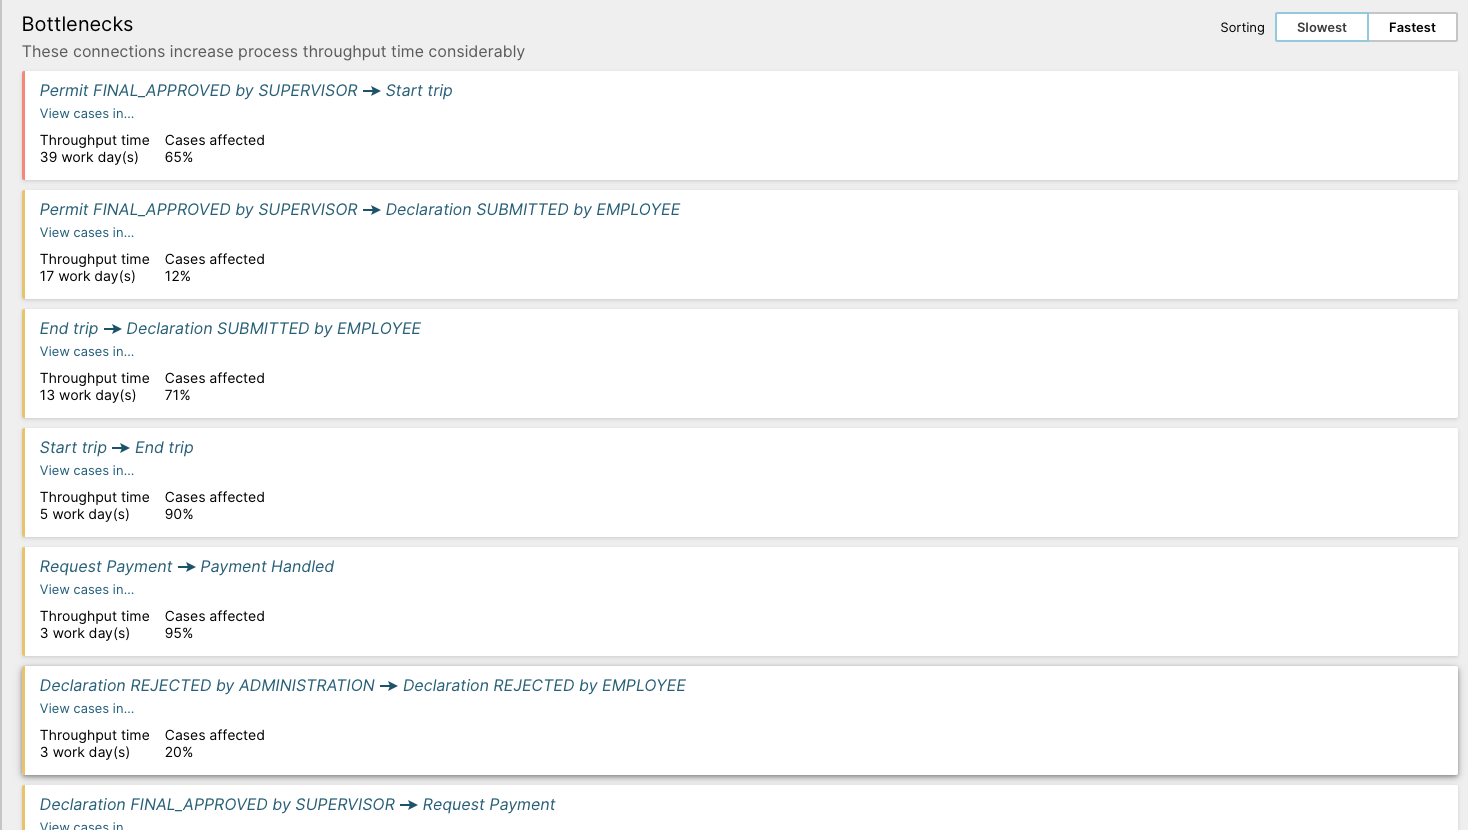
\includegraphics[width=\textwidth]{figures/celonis/int_bottlenecks.png}
		\caption{International}
	\end{subfigure}
	\caption{Langsamste Aktivitätsübergänge laut Celonis-Bottleneck-Analyse (in Arbeitstagen)}
	\label{fig:bottlenecks}
\end{figure}

% ==================================================================
\subsection{Ablehnungen und Rework-Schleifen}
\label{sec:rejections}

Die Auswertung im eigens konzipierten \textit{Rejections Dashboard} (siehe \autoref{fig:view_rejections} im Anhang) zeigt, dass Ablehnungen ein massives Effizienzproblem darstellen: Im Domestic-Log sind insgesamt 1.301 von 10.500 Fällen (12\,\%) von mindestens einer Ablehnung betroffen; im komplexeren International-Log steigt diese Quote um mehr als das Doppelte auf 1.755 von 6.449 Fällen (27\,\%), wobei dort sowohl die vorgelagerten Permits als auch die nachgelagerten Declarations abgelehnt werden können.

Auf Ebene der prüfenden Instanzen dominiert die Verwaltung (\texttt{ADMINISTRATION}), die in 846 Domestic-Cases (8\,\%) und 1.287 International-Cases (20\,\%) eine Ablehnung ausspricht, gefolgt vom \texttt{SUPERVISOR} (281 Domestic-Cases, 3\,\%) sowie selteneren Zurückweisungen durch \texttt{PRE\_APPROVER} (81 Cases), \texttt{BUDGET OWNER} (58 Cases), \texttt{DIRECTOR} und eine nicht näher spezifizierte Rolle \texttt{MISSING} (87 Domestic-Cases). Da die Gesamtzahl der protokollierten Ablehnungs-Events die Anzahl der betroffenen Cases deutlich übersteigt (z.\,B.\ 952 Admin-Ablehnungs-Events verteilt auf 846 Cases bei Domestic bzw.\ 1.549 Events auf 1.287 Cases bei International), durchlaufen zahlreiche Anträge mehrfache Zurückweisungsschleifen.

\paragraph{Aufklärung der Aktivität \enquote{Rejected by EMPLOYEE}.}
Quantitativ tritt in beiden Logs die Aktivität \texttt{Declaration REJECTED by EMPLOYEE} mit 1.212 Fällen (12\,\%, Domestic) bzw.\ 1.483 Fällen (23\,\%, International) am häufigsten auf. Durch eine gezielte Filterung auf die 1.301 abgelehnten Domestic-Cases im selbsterstellten Celonis-View (\autoref{fig:view_rejections} im Anhang) lässt sich die tatsächliche Prozesssemantik dieser zunächst widersprüchlich klingenden Aktivität eindeutig klären: Sie tritt im Prozessgraphen nahezu ausnahmslos als unmittelbarer Folgeschritt nach einer Ablehnung durch die Administration, den Supervisor oder den Budget Owner auf (im International-Log im Mittel nach 3 Arbeitstagen, vgl.\ \autoref{fig:bottlenecks}). Eine Überprüfung konkreter Einzelfälle im \textit{Case Explorer} – etwa Case \texttt{ff999942-a443-4452-9b09-3c5e60ee3a8f}, bei dem exakt sieben Stunden nach \texttt{Declaration REJECTED by SUPERVISOR} das Event \texttt{Declaration REJECTED by EMPLOYEE} folgt – belegt, dass Mitarbeitende hier nicht ihren eigenen Antrag prüfen, sondern dass das Workflow-System einen vom Prüfer abgelehnten Antrag formal mit dem Status \texttt{REJECTED by EMPLOYEE} an den Einreicher zurückspielt (bzw.\ dieser die Kenntnisnahme/Stornierung bestätigt). Von diesem Knotenpunkt aus teilt sich der Prozessfluss im Dashboard in zwei Pfade: Entweder reicht der Mitarbeitende den korrigierten Antrag erneut ein (Rückwärtsschleife zu \texttt{Declaration SUBMITTED by EMPLOYEE}), oder der Prozess bricht an dieser Stelle endgültig ab.

\paragraph{Rework-Effekt und Prozessabbruch.}
Wird nach einer Ablehnung eine Korrekturschleife durchlaufen, führt dies zu erheblichem Mehraufwand (\textit{Rework}). In 776 Domestic-Cases (7\,\%) und 1.225 International-Cases (19\,\%) wird eine Deklaration mehrfach eingereicht, was die Durchlaufzeit im Mittel um 12 bzw.\ 20 Tage verlängert und 3,6 bzw.\ 4,6 zusätzliche Prozessschritte verursacht (\autoref{fig:violations}). Im Einzelfall zeigt sich in den Zeitstempeln, dass reine Formalkorrekturen nach der Wiedereinreichung oft in wenigen Sekunden von der Administration durchgewunken werden (im untersuchten Case \texttt{f954cbea...} dauerte die Freigabe nach der Zweiteinreichung exakt 6 Sekunden), die vorangegangene Schleife jedoch Wochen an Liegezeit gekostet hat.

Gleichzeitig zeigt die Filterung auf die 1.301 abgelehnten Domestic-Cases im Prozessgraphen (\autoref{fig:view_rejections} im Anhang), dass 979 dieser Fälle (75\,\% der abgelehnten Fälle) nach erfolgreicher Korrektur dennoch den Endknoten \texttt{Payment Handled} erreichen. Die verbleibenden 322 abgelehnten Fälle enden hingegen ohne Auszahlung. Zusammen mit den 134 nie eingereichten Entwürfen (\texttt{SAVED by EMPLOYEE}) erklärt dies exakt die insgesamt 456 Domestic-Cases (4,3\,\%), in denen kein \texttt{Payment Handled} stattfindet (10.044 bezahlte von 10.500 Fällen). Im International-Log bleiben analog 190 Cases ohne Auszahlung (6.259 bezahlte von 6.449 Fällen).

\paragraph{Analyse potenzieller Ablehnungsgründe.}
Inhaltliche Ablehnungsgründe (wie bspw.\ fehlende Originalbelege, falsch berechnete Tagessätze oder unzulässige Ausgabenkategorien) werden im Event-Log nicht als explizites Textattribut erfasst.
Der direkte XES-Upload in Celonis übernimmt standardmäßig lediglich die Event-Ebene (\texttt{id}, \texttt{org:resource}, \texttt{concept:name}, \texttt{time:timestamp}, \texttt{org:role}) in die zentrale Aktivitätstabelle (vgl.\ Abbildung~\ref{fig:anhang-datenmodell}).
Die auf Case-Ebene liegenden Metadaten, etwa die Betragsfelder \texttt{Amount}, \texttt{RequestedAmount}, \texttt{AdjustedAmount} oder \texttt{OriginalAmount}, stehen im Standard-Import nicht als Case-Attribute für PQL-Abfragen zur Verfügung.
Dieses Verhalten deckt sich mit einem dokumentierten Feature-Request in der Celonis Community, wonach Trace-Attribute beim XES-Import auf Event-Ebene abgeflacht werden und keine separate Case-Tabelle entsteht \parencite{buijs2019celonis}.
Diese technische Restriktion schränkt die automatisierte Ursachenanalyse in Celonis ein.
Zwar ließe sich die Einschränkung durch eine vorgelagerte Konvertierung der Ereignisprotokolle in das CSV-Format und einen strukturierten Relational-Datenimport umgehen, bei dem sämtliche Fallattribute in das Datenmodell integriert würden; diese Erkenntnis wurde im Verlauf des Analyseprozesses jedoch erst gewonnen, als die Dashboards und Kennzahlen bereits auf Basis des nativen XES-Imports etabliert waren.
Die strukturierte Untersuchung von Ablehnungsursachen musste daher auf die in Celonis nativ verfügbaren Ablaufstrukturen, Rollen und Schleifenmuster beschränkt bleiben.

% ==================================================================
\subsection{Unerwartetes Verhalten}
\label{sec:unerwartet}

\paragraph{Fehlende Reiseanträge (Missing Permits).}
Obwohl für Auslandsreisen zwingend eine Vorabgenehmigung vorgeschrieben ist, starten 748 International-Cases (12\,\%) unmittelbar mit der Aktivität \texttt{Start trip}. Diese Regelverletzung verlängert die Gesamtdurchlaufzeit im Schnitt um 29 Tage (\autoref{fig:violations}). Ein Abgleich mit den Gesamtfallzahlen präzisiert das Bild: Da überhaupt nur 6.001 der 6.449 Fälle das Event \texttt{Permit SUBMITTED by EMPLOYEE} aufweisen, existieren genau 448 Auslandsreisen (7\,\%), die den gesamten Abrechnungsprozess ohne jemals eingereichten Reiseantrag durchlaufen – exakt jene 448 Fälle, die bereits in der Attributanalyse (\autoref{sec:datensatzuebersicht}) durch den Dummy-Eintrag \enquote{\texttt{travel permit 423}} im Feld \texttt{Permit id} aufgefallen waren. In den übrigen rund 300 der 748 Fälle wird das Permit erst nach Reiseantritt eingereicht.

\paragraph{Nachträglich genehmigte Reisen.}
Selbst wenn ein Permit gestellt wird, erfolgt die Genehmigung häufig zu spät. Wie in der Bottleneck-Analyse (\autoref{sec:bottlenecks}) beobachtet, folgt in 776 International-Cases (12\,\%) auf \texttt{Permit FINAL\_APPROVED by SUPERVISOR} direkt die Einreichung der Abrechnung (\texttt{Declaration SUBMITTED by EMPLOYEE}, 17\,AT), ohne dass dazwischen Reise-Events liegen. Eine Detailprüfung der Zeitstempel dieser 776 Fälle belegt eine massive Umgehung des Kontrollprinzips:
\begin{itemize}[noitemsep]
	\item In 582 Fällen (75\,\%) war die Dienstreise (\texttt{Start trip} bis \texttt{End trip}) bereits \emph{vollständig beendet}, bevor die finale Permit-Genehmigung erteilt wurde (488 davon begannen direkt mit \texttt{Start trip}).
	\item In 53 Fällen (7\,\%) fiel die Genehmigung in den laufenden Reisezeitraum.
	\item Lediglich in 141 Fällen (18\,\%) wurde die Kostenerklärung regulär vor Reisebeginn eingereicht (etwa zur Voraberstattung gebuchter Flüge oder Konferenzgebühren).
\end{itemize}
Die Reisegenehmigung verkommt in über vier Fünfteln dieser Fälle von einer präventiven Budgetkontrolle zu einer rein bürokratischen Nachgenehmigung, die nur noch durchlaufen wird, um die Auszahlung im System freizuschalten.

\paragraph{Zusätzliche Eskalationsstufen.}
In exakt 637 International-Cases (10\,\%) treten die Aktivitäten \texttt{Permit APPROVED by SUPERVISOR} und \texttt{Permit FINAL\_APPROVED by DIRECTOR} auf. Die identische Fallzahl belegt, dass der Supervisor hier nur eine Vorprüfung vornimmt und die Endfreigabe an die Direktoratsebene eskaliert wird. Mit einer mittleren Verzögerung von +52 Tagen stellt diese Eskalationsstufe den größten einzelnen Zeittreiber im gesamten Datensatz dar (\autoref{fig:violations}).

\paragraph{Unprotokollierte Neueinreichungen.}
Im Domestic-Log folgt in 193 Fällen (2\,\%) auf eine bereits erfolgte Verwaltungsfreigabe (\texttt{Declaration APPROVED by ADMINISTRATION}) unmittelbar ein erneutes \texttt{Declaration SUBMITTED by EMPLOYEE} (+12\,d, +4,9 Schritte), ohne dass dazwischen ein Ablehnungs-Event protokolliert ist. Dies deutet darauf hin, dass Mitarbeitende bereits geprüfte Anträge aktiv zurückziehen oder nachträglich Belege nachreichen können, was den Prüfprozess von vorn anstößt.

\begin{figure}[htbp]
	\centering
	\begin{subfigure}[t]{0.49\textwidth}
		\centering
		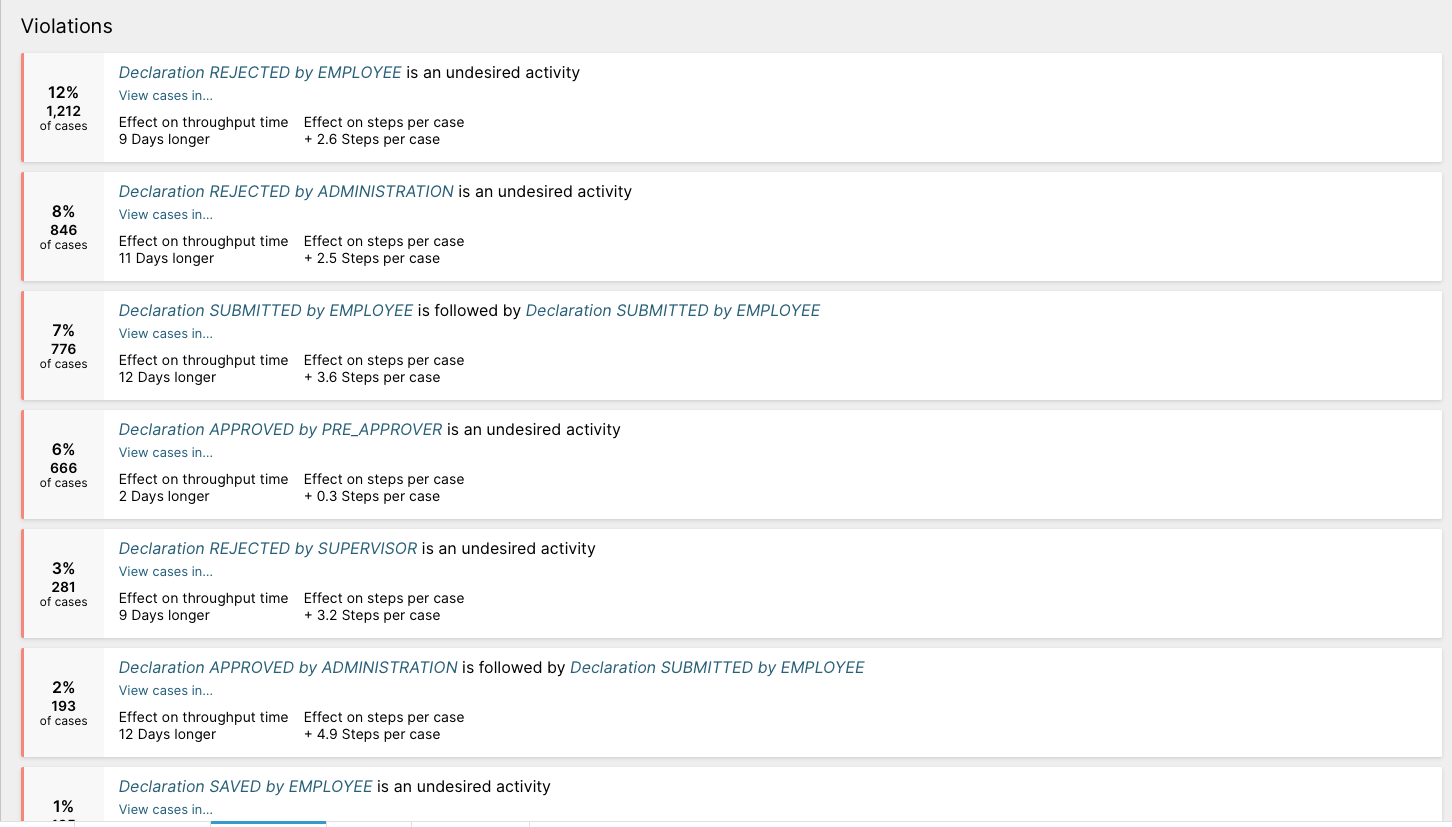
\includegraphics[width=\textwidth]{figures/celonis/dom_violations.png}
		\caption{Domestic}
	\end{subfigure}
	\hfill
	\begin{subfigure}[t]{0.49\textwidth}
		\centering
		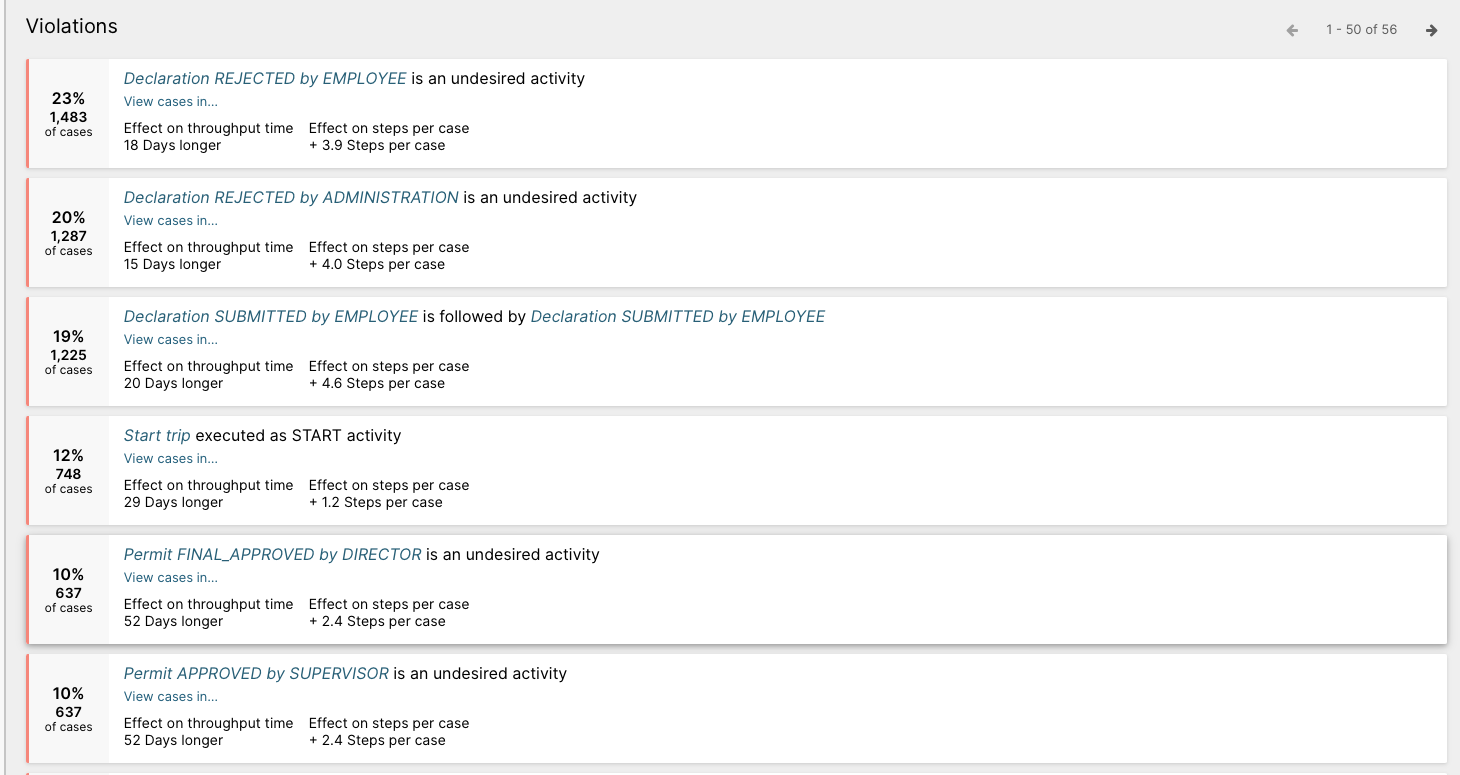
\includegraphics[width=\textwidth]{figures/celonis/int_violations.png}
		\caption{International}
	\end{subfigure}
	\caption{Häufigste Abweichungen vom Referenzmodell mit Effekt auf Durchlaufzeit und Schrittanzahl (Celonis \textit{Conformance})}
	\label{fig:violations}
\end{figure}

% ==================================================================
\subsection{Muster mangelnder Konformität}
\label{sec:nonconformance}

Conformance Checking gleicht das im Event-Log beobachtete Verhalten systematisch mit einem Prozessmodell ab \parencite{carmona_conformance_2018}. Eine zentrale methodische Erkenntnis dieser Untersuchung ist, dass die gemessene Konformitätsquote sowie ihre zeitliche Entwicklung unmittelbar von der Wahl und dem Abstraktionsgrad des zugrundeliegenden Referenzmodells abhängen. Um diesen Effekt nachzuweisen, wurde das Conformance Checking in Celonis zweistufig durchgeführt (\autoref{fig:conformance_comparison} sowie \autoref{tab:kpi_comparison}):

\begin{enumerate}[noitemsep]
    \item \textbf{Striktes Happy-Path-Modell (nur Variante 1):} Wird im Domestic-Log ausschließlich die häufigste Prozessvariante als Soll-Modell definiert (\autoref{fig:conf_model_strict}), beträgt die Gesamtkonformität exakt 44\,\% (4.618 Cases) (\autoref{fig:conf_hist_strict}). Der zeitliche Verlauf offenbart dabei ein extremes Muster: Von Januar bis Oktober 2017 liegt die Konformitätsquote bei $\approx 0\,\%$ und springt erst im Januar 2018 unvermittelt auf konstant 55--60\,\%.
    \item \textbf{Erweitertes Kernmodell (Top-3-Varianten mit XOR-Gateways):} Werden über exklusive Gateways (XOR) zusätzlich die Freigabe durch den \texttt{BUDGET OWNER} (Variante 2, 23\,\%) sowie das Überspringen der Administration (Variante 3, 13\,\%) als optionale Pfade zugelassen (\autoref{fig:conf_model_top3}), steigt die Gesamtkonformität auf 81\,\% (8.470 Cases). Gleichzeitig erhöht sich die Konformität im Jahr 2017 sprunghaft auf 50--75\,\% und erreicht ab Januar 2018 Werte zwischen 80\,\% und 90\,\% (\autoref{fig:conf_hist_top3}).
\end{enumerate}

Ein völlig analoges Bild zeigt sich im International-Log: Gegenüber dem strikten Happy-Path-Modell (21\,\% Gesamtkonformität, 1.369 Cases) liegt die Konformität bis einschließlich Dezember 2017 ebenfalls bei 0\,\% und steigt erst im erweiterten Modell (Top-3-Varianten mit XOR-Verzweigungen für Administration und Budget Owner) auf insgesamt 38\,\% (2.470 Cases; 20--35\,\% in 2017 vs.\ 40--47\,\% ab 2018; siehe \autoref{fig:conformance_comparison_int} im Anhang).

\begin{figure}[htbp]
    \centering
    % --- Obere Zeile: BPMN-Referenzmodelle ---
    \begin{subfigure}[t]{0.49\textwidth}
        \centering
        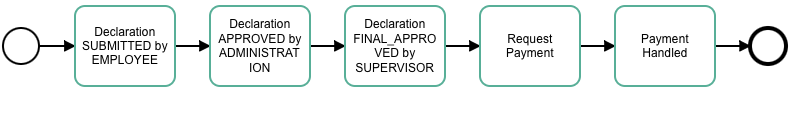
\includegraphics[width=\textwidth]{figures/celonis/dom_bpmn_v1.png}
        \caption{Striktes Happy-Path-Modell (nur Variante 1)}
        \label{fig:conf_model_strict}
    \end{subfigure}
    \hfill
    \begin{subfigure}[t]{0.49\textwidth}
        \centering
        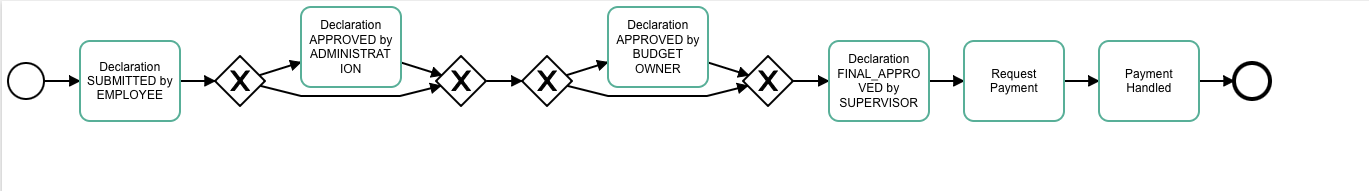
\includegraphics[width=\textwidth]{figures/celonis/dom_bpmn_top3.png}
        \caption{Erweitertes Kernmodell (Top-3-Varianten mit XOR)}
        \label{fig:conf_model_top3}
    \end{subfigure}

    \vspace{0.4cm}

    % --- Untere Zeile: Zugehörige Conformance-Verläufe ---
    \begin{subfigure}[t]{0.49\textwidth}
        \centering
        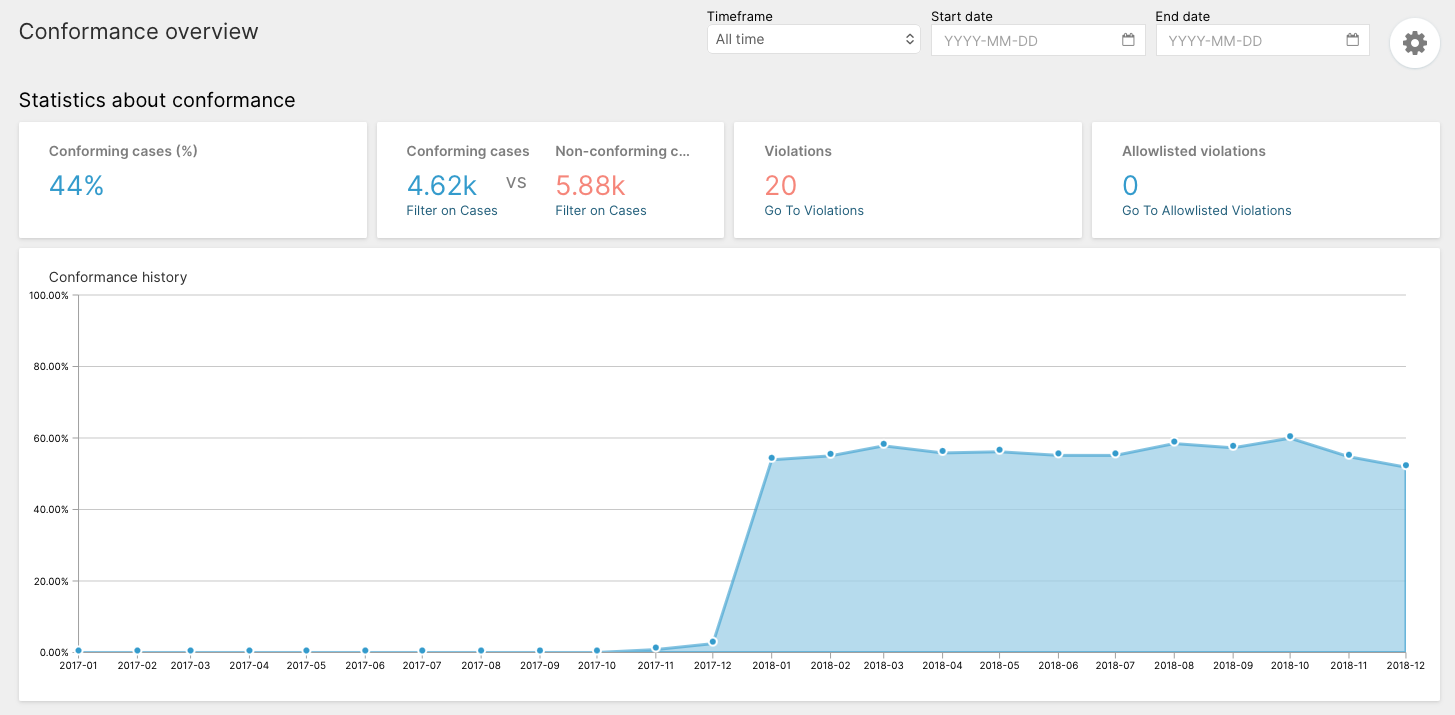
\includegraphics[width=\textwidth]{figures/celonis/dom_conf_v1.png}
        \caption{Konformitätsverlauf bei striktem Happy Path (44\,\%)}
        \label{fig:conf_hist_strict}
    \end{subfigure}
    \hfill
    \begin{subfigure}[t]{0.49\textwidth}
        \centering
        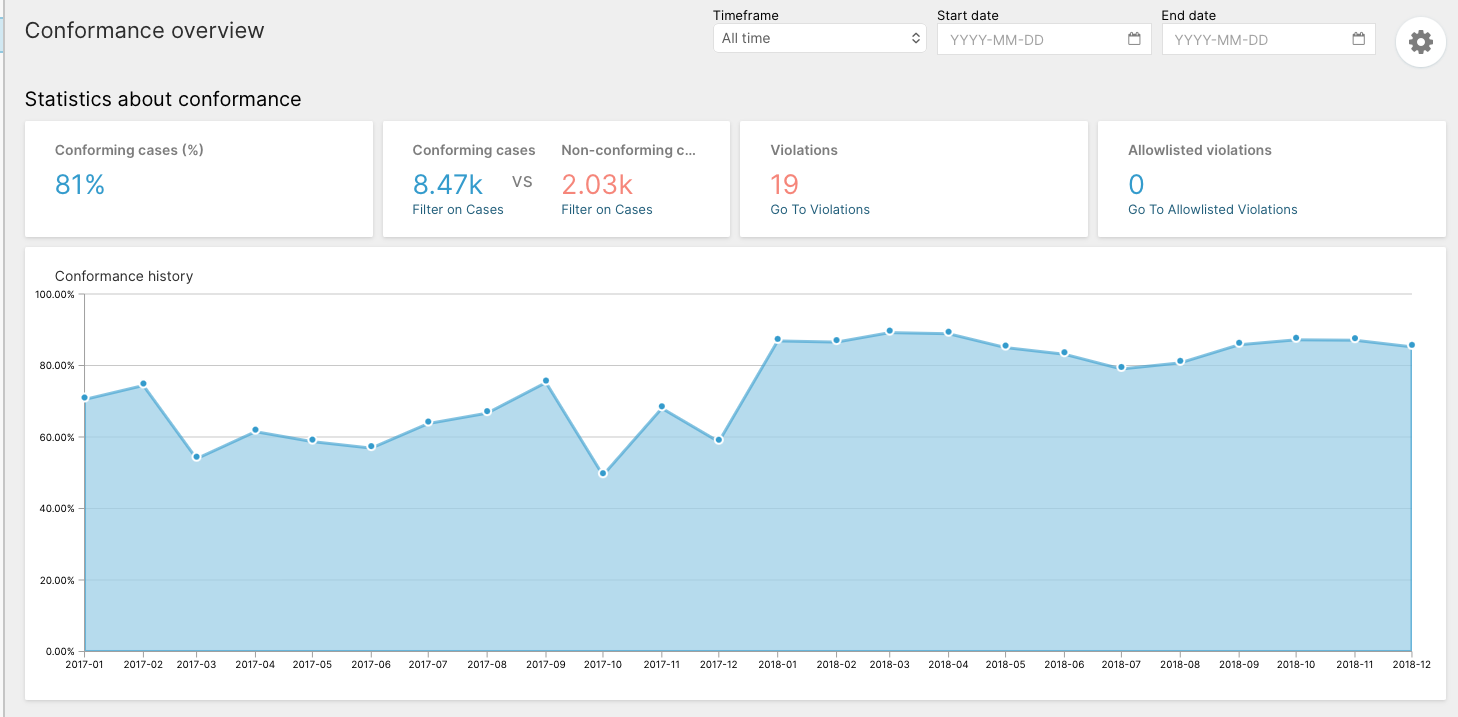
\includegraphics[width=\textwidth]{figures/celonis/dom_conf_top3.png}
        \caption{Konformitätsverlauf bei Top-3-Varianten (81\,\%)}
        \label{fig:conf_hist_top3}
    \end{subfigure}

    \caption{Einfluss des Referenzmodells auf die gemessene Konformität im Domestic-Log (links: nur Variante 1 mit $\approx 0\,\%$ Konformität in 2017; rechts: Top-3-Varianten inkl.\ Budget Owner)}
    \label{fig:conformance_comparison}
\end{figure}

\paragraph{Zeitlicher Verlauf und das Rollout-Artefakt 2018.}
Aus diesem Modellvergleich lassen sich zwei zentrale Schlüsse über die Prozesslandschaft der Universität ziehen. Erstens existierte der globale \enquote{Happy Path} (Variante 1) im Jahr 2017 in den beiden zuerst erfassten Pilotfakultäten faktisch nicht; dort durchliefen sämtliche Abrechnungen zwingend entweder einen \texttt{BUDGET OWNER}, einen \texttt{PRE\_APPROVER} oder übersprangen die Administration. Zweitens erklärt sich der markante Konformitätsanstieg zum Januar 2018 in beiden Logs nicht durch eine plötzliche operative Prozessverbesserung, sondern durch die Ausweitung der Datenerfassung auf die gesamte Universität \parencite{van_dongen_bpi_2020}. Da das Jahr 2018 rund viermal so viele Fälle umfasst wie das Pilotjahr 2017 (\autoref{tab:basisstatistik}), dominieren die neu angeschlossenen Fakultäten – in denen der schlanke Prozess ohne Budget Owner den Standard bildet – die Häufigkeitsverteilung des Gesamt-Logs. Ein datengetrieben aus den häufigsten Varianten generiertes Referenzmodell unterliegt somit einem Mengen-Bias zugunsten des Jahres 2018 und stuft abweichende Fakultätsprozesse aus 2017 systematisch häufiger als nicht konform ein.

\paragraph{Deskriptive vs.\ normative Modellgrenzen.}
Zugleich verdeutlicht das erweiterte Kernmodell (81\,\% bzw.\ 38\,\% Konformität) den Unterschied zwischen einem \emph{deskriptiven} (frequenzbasierten) und einem \emph{normativen} (regelgetriebenen) Referenzmodell: Ob eine Aktivität in Celonis als Regelverletzung (\enquote{undesired activity}) gewertet wird, hängt hier allein davon ab, ob sie in den ausgewählten Top-Varianten enthalten ist. Während die Freigabe durch den \texttt{BUDGET OWNER} (27--28\,\% der Cases) durch die Aufnahme der Varianten 2 und 3 als konform gilt, wird die fachlich vergleichbare Vorprüfung durch den \texttt{PRE\_APPROVER} (6\,\%, 666 Cases) als Verletzung gezählt (\autoref{fig:violations}), obwohl auch sie einen legitimen organisatorischen Prüfschritt darstellt. Die Allowlist von Celonis wurde bewusst nicht genutzt (0 allowlisted violations), um diese unverzerrten Rohwerte offenzulegen. Umgekehrt dürfte das automatisch generierte BPMN-Modell in Celonis aber auch nicht unkritisch auf weitere Varianten (z.\,B.\ Top-5) ausgeweitet werden: In diesem Fall würden auch Ablehnungsschleifen (\texttt{Declaration REJECTED by ADMINISTRATION} $\rightarrow$ \texttt{REJECTED by EMPLOYEE}) über ein XOR-Gateway als regulärer Modellpfad aufgenommen, wodurch echte Prozessfehler fälschlicherweise als \enquote{konform} eingestuft würden.

\paragraph{Zusammenfassung der Non-Conformance-Muster.}
Unter Berücksichtigung dieser Modellcharakteristik identifiziert Celonis im erweiterten Kernmodell 19 Verletzungstypen im Domestic- und 56 im International-Log. Nicht konforme Fälle dauern im Mittel 5,9 Tage (16,3 vs.\ 10,4\,d, Domestic) bzw.\ 27,8 Tage (97,1 vs.\ 69,3\,d, International) länger und erfordern durchschnittlich 1,3 bis 1,6 zusätzliche Prozessschritte (\autoref{tab:kpi_comparison}). Inhaltlich verdichten sich die Abweichungen auf vier zentrale Muster:

\begin{enumerate}[noitemsep]
    \item \textbf{Rework-Schleifen:} Ablehnungen mit anschließender Korrektur und Neueinreichung (\autoref{sec:rejections}) bilden in beiden Logs die häufigste und zeitintensivste Abweichung.
    \item \textbf{Umgehung der Vorab-Genehmigungspflicht:} 12\,\% der Auslandsreisen starten gänzlich ohne eingereichtes Permit; in weiteren Fällen wird die Genehmigung erst nach Reiseende eingeholt (\autoref{sec:unerwartet}).
    \item \textbf{Verzögerte Einreichung:} Deklarationen werden nach Reiseende erst mit erheblichem Verzug (Ø 13 Arbeitstage) eingereicht (\autoref{sec:bottlenecks}).
    \item \textbf{Zusätzliche Eskalations- und Prüfstufen:} Die Einbindung von \texttt{PRE\_APPROVER} und \texttt{DIRECTOR} verlängert die Durchlaufzeit signifikant (bis zu +52\,d) und wird vom frequenzbasierten Modell als Verletzung markiert, stellt fachlich jedoch meist einen regelkonformen Sonderpfad dar.
\end{enumerate}
